\chapter{Introdução}\label{cap:01}

Desde que as pinturas começaram, se formaram vários estilos de arte, ainda que no princípio tudo era voltado a chegar ao realismo das pinturas, por não existir nada que pudesse retratar rostos e momentos melhor do que as artes.

No entanto, isso mudou quando surgiram as câmeras, que poderiam captar tudo de forma praticamente instantânea, com isso era o momento de se pensar que as pinturas iriam sumir, mas ela se renovou e ao invés de buscar o realismo, agora ela estava em busca de trazer novas sensações, como as pinturas abstratas, estilos como cubismo ou surrealismo que usavam de várias curvas e cores para demonstrar expressões \cite{debora_2021}.

Esses estilos artísticos foram uma revolução no mundo da arte, como o surrealismo por exemplo, que tratava de possibilidades infinitas em suas obras, porque ali tudo era possível e o único limite era imaginação, Nesse período foram apresentadas várias obras que ao olhar não faziam sentido algum, porém era esse o princípio da ideia, pois elas eram criadas para passar uma sensação a quem olhasse, como a de liberdade, entre outros.

Atualmente a iluminação é de extrema importância para as  pinturas e desenhos digitais pois é ela quem traz o volume ao ambiente, como pode ser observado na Figura 1.

\begin{figure}[h]
	\caption{Duas imagens demonstrando a diferença da iluminação }
	\centering
	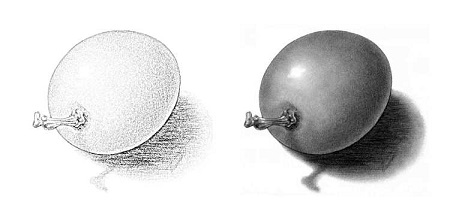
\includegraphics{imagens/luz-e-sombra-para-produzir-volume.jpg}\cite{Grafitti_2019}
\end{figure}


Como podemos observar que na figura acima, a imagem da esquerda apresenta apenas um rascunho, sem uso das técnicas de iluminação a portanto a noção de volume e profundidade não fica muito claro, por outro lado a imagem da direita sendo algo mais agradável nas pinturas como é possível notar, além do mais várias composições de cores da luz retratada em uma imagem pode trazer vislumbres fantásticos.

Com a chegada dos primeiros modelos em três dimensões, como cubos, piramides e esferas entre outros, foi possível enxergar através de uma tela, um objeto qualquer que fosse e isso mudou tudo, hoje podemos ver vários exemplos de modelos que está em nossa realidade, como a impressora 3D ou o \textit{Billboard}\footnote{apresentado em Tóquio, uma televisão imensa que pode captar imagens como se fossem 3D, criando um aspecto de profundidade pela sua curvatura}, pois é com ela que foi possível ver a grande beleza dos modelos, é por esse motivo pelo qual atualmente a iluminação é essência para nos causar a sensação de volume, sem pensar nos algoritmos mais robustos como \textit{ray tracing} que segundo \citeonline{shirley_2008} retrata, é um algoritmo onde através de uma janela, os raios são direcionados para as imagens. As superfícies são perdidas ou atingidas por cada pixel, que é representado por um raio. Ao atingir uma superfície, o raio se refrata e continua em um novo curso, causando a formação de luzes adicionais nos arredores.

Porém para os artistas chegarem perto dos algoritmos de iluminação que criam visuais impecáveis em três dimensões, as pinturas e artes foram obrigadas a criar um volume e melhorar a iluminação, pois como a luz funcionava de forma sistemática em três dimensões, as artes puderam abrir espaço em uma variação de cores e paletas diferenciadas que trazem um dinamismo maior.

Por isso atualmente a iluminação se tornou algo tão importante para o mundo, que não importa mas o estilo que é usado, é uma parte essencial. É nesse momento em que chegamos ao cerne do problema, pois com essa importância que a iluminação tem sobre a arte e os avanços tecnológicos cada vez mais ligados a ter um \textit{design} rápido e com eficiência, ferramentas que criam a luz em pinturas, desenhos, objetos, \textit{sprites} ou até logos poderia impactar a arte de maneira eficiente e até mesmo para aumentar a comunidade, fazendo com que várias pessoas iniciantes que não conseguem bons resultados possam aparecer no mundo do \textit{design}.

\section{Objetivos}

\subsection{Objetivo Geral}
O objetivo do trabalho é simular a iluminação em imagens digitais de média e baixa resolução por meio do desenvolvimento de uma ferramenta.

%O objetivo do trabalho é criar uma ferramenta que possa, a partir de uma imagem qualquer, gerar um ambiente tridimensional que irá simular a iluminação de forma natural.

\subsection{Objetivos Específicos}
\begin{itemize}
	\item Encontrar algoritmos que têm o propósito de iluminar cenas bidimensionais;
	\item Criar um protótipo e desenvolver a ferramenta para iluminação;
	\item Realizar testes na ferramenta Relight que será analisado para comparação dos resultados.
\end{itemize}